\begin{itemize}
\item{\textbf{Kratak opis:} Vozach prijavljuje kvar vozila na putu popunjavanjem formulara u okviru sistema.}
\item{\textbf{Akteri:} Vozach}
\item{\textbf{Ulaz:} Podaci o vozilu, lokaciji i opis kvara }
\item{\textbf{Izlaz:} Poruka o uspeshnosti prijave kvara }
\item{\textbf{Preduslovi:} Vozach ima pristup sistemu i poseduje potrebne informacije o vozilu. }
\item{\textbf{Postuslovi:} Uspeshno prijavljen kvar.}
\item{\textbf{Glavni tok:} Vozach unosi traz1ene podatke preko formulara za prijavu kvara u okvirusistema (naziv i tip vozila, ID vozila, registracioni broj vozila, tachna lokacija i opis kvara). Sistem obradjuje podatke i az1urira stanje. Nakon toga prikazuje se potvrda o uspeshnosti prijavljivanja kvara. }
\item{\textbf{Alternativni tokovi:} Neuspeshno prijavljivanje kvara.}
\end{itemize}
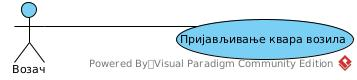
\includegraphics{Slike/SUodrzavanje.jpg}